
\section{Design}

\subsection{High Level Design}

The program runs on a server equipped with a GPU and is accessed through an HTML webpage, in order to guarantee performance for users without high performance graphics cards. The webpage offers two high-level functions which rely on each other:
\begin{enumerate}
\item \label{it:seg} Making fast and accurate segmentations of medical images on both seen and unseen object types using some pre-trained AI and with the help of user interaction
\item \label{it:transfer} Adding correct segmentations to a dataset in order to train a new or pre-existing AI to perform better segmentations
\end{enumerate}

That is to say, function \ref{it:seg} produces the data for function \ref{it:transfer} to train on, and function \ref{it:transfer} trains an AI that can be used by function \ref{it:seg} to produce better results. The method for performing function \ref{it:seg} is, in a high-level form, identical to that of Wang et al. in the BIFSeg paper \cite{BIFSeg} (section \ref{BIFSeg}), but some of the internal components have been changed and modified, namely
\begin{itemize}
\item The CNN architecture
\item The CNN loss function
\item The algorithm for optimizing the CRF
\item The values of various hyperparameters
\end{itemize}

For function \ref{it:transfer}, we use transfer learning to minimize training times. When the user creates a new CNN for an unseen object class, the CNN used in generalized segmentation and it's weights are copied over and a corresponding dataset is also created on the server. Every time the user segments an image, they can upload the image and corresponding segmentation to the dataset, and when there are enough images, they can train the new CNN on the dataset. This then makes further segmentations much faster since initial predictions will be much more accurate and thus will need less user interaction. The motivations behind transfer learning are explained in section \ref{sec:transferLearn}.

\begin{figure}[h!]
\centering
\makebox[\textwidth][c]{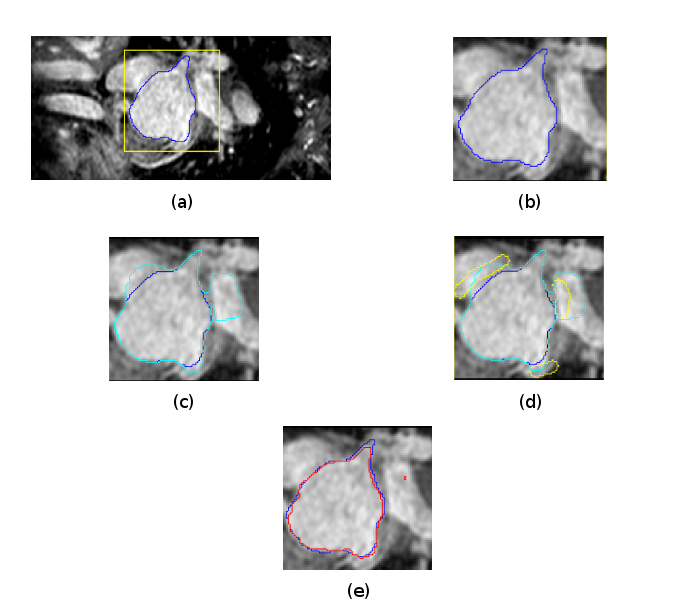
\includegraphics[scale=0.65]{pictures/BIFSegEx}}
\caption{5 images showing the process of segmenting the left atrium from an image. In blue is the ground truth, (i.e. the left atrium), in cyan is the initial guess of the CNN+CRF, in yellow are user scribbles labelling pixels as background and in red is the final segmentation. Only a single 2D slice is shown, but the full image is a 3D volume}
\label{fig:BIFSegEx}
\end{figure}


The process for producing segmentations goes as follows, and is also shown in figure \ref{fig:BIFSegEx}:
\begin{enumerate}
\item \label{it:first} The user opens the webpage and loads an image in NIFTI format which is displayed with a set of images along each of the 3 axis of the volume
\item \label{it:CNN} The user selects a CNN, either one trained specifically for the object at hand or one trained in general segmentation
\item The user draws a bounding box around the area of interest (figures \ref{fig:BIFSegEx}a and \ref{fig:BIFSegEx}b)
\item The CNN makes a prediction which is refined by the CRF and presented to the user (figure \ref{fig:BIFSegEx}c)
\item \label{it:scribb} The user provides "scribbles" for the CNN, labelling pixels correctly, particularly in regions which are currently mislabeled (figure \ref{fig:BIFSegEx}d)
\item \label{it:BIFSeg} The following steps are then repeated some fixed number of times:
\begin{enumerate}
\item A weight array is produced to weigh the loss function on a per-pixel basis. Scribbles are overweighted by some factor $w>1$. Uncertain pixels and those that are geodesically near a scribble of opposite binary value are given 0 weight. 
\item The CNN is trained to fit the segmentation, with the loss function weighted by the weight array
\item A segmentation is produced using the trained CNN and the CRF (with the scribbles)
\end{enumerate}
\item \label{it:fin} The final segmentation is presented to the user (figure \ref{fig:BIFSegEx}e). If the user does not consider it good enough, they can easily add extra scribbles to help the AI, repeating steps \ref{it:scribb} and \ref{it:BIFSeg}. The user can also manually alter the segmentation
\item \label{it:transfer2} At this point the user may add the image and its segmentation to a new or already existing dataset. If they consider the dataset to be large enough, they can then train the corresponding CNN on its dataset, and which point they can choose this CNN in step \ref{it:CNN} when they segment the next image.
\item Repeat steps \ref{it:first}-\ref{it:transfer2} for each desired image
\end{enumerate}




\subsection{CNN}

We train 2 CNNs, the first of which is trained on a specific organ in order to test performance on seen images. The second will be a CNN trained in generalized segmentation, in order to test the performance on unseen objects and the performance of transfer learning. It will therefore be trained on a variety of organs.

\subsubsection{Architecture}

\begin{figure}[h!]
\centering
\makebox[\textwidth][c]{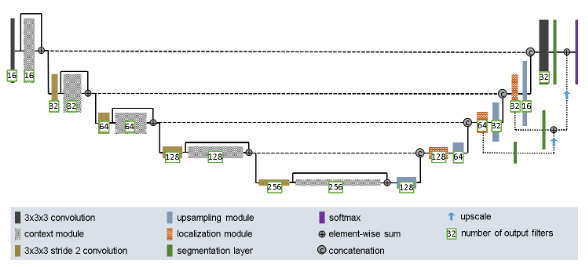
\includegraphics[scale=0.75]{pictures/isensee}}
\caption{A diagram of the Isensee et al. model, inspired by U-Net but with residual connections, spatial dropout and segmentation layers to encourage good segmentation earlier in the model \cite{UResNet}}
\label{fig:isensee}
\end{figure}

The architecture used is that developed by Isensee et al. \cite{UResNet} (see figure \ref{fig:isensee}) which achieved state of the art results in the Brain Tumour Segmentation challenge by improving on the standard U-Net architecture. The network uses residual blocks to improve the learning speed and performance and uses spatial dropout to avoid overfitting. It also has segmentation layers, extra connections that upsample and then sum that outputs from the layers of varying coarseness on the right hand side of the U shape. The final segmentation is then a sum of the output of these various layers, which works to encourage the connected layers of different coarseness to all produce segmentations. This should encourage the network to learn as we expect it to, with coarser segmentations being combined with finer feature maps outputting progressively finer segmentations. The CNN also uses strided convolution rather than pooling in order to increase the size of the receptive field. The CNN is built in Keras using Tensorflow backend, and uses parts of the code produced by David Ellis \cite{uNetGit}.

We use this model as we find it to be faster than the PC-Net used by Wang et al. in BIFSeg, while still maintaining a state of the art performance. Each weight matrix at each layer is convolved over every feature in the feature map, and since PC-Net does not reduce the size of the feature map via pooling layers, this causes inference and backpropagation to take longer. 

During fine-tuning, we only fine-tune the segmentation side (right hand side) of the U-shape. However, due to time constraints, we have not yet implemented the saving of the outputs of the untrained part, as done by Wang et al. which will reduce fine-tuning time significantly.

\subsubsection{Loss function}

Class imbalance is an issue with regards to the loss function, most images have far more background pixels than foreground pixels, thus the network tends to skew its predictions. The naive cross-entropy that Wang et al. use suffers from this problem. Inspired by the Dice score, Isensee et al. define the weighted dice coefficient $D_c$ as

\begin{equation}
D_c = \frac{1}{K} \sum_{k} \frac{2\sum_{i} o^{k}_i y^{k}_i}{\sum_{i} o^{k}_i + \sum_{i} y^{k}_{i}}
\end{equation}

where $o^{k}_i$ is the network output for the kth class on the ith pixel, $y^{k}_{i}$ is the target output, and $K$ is the number of classes. We can easily turn this dice coefficient into a dice coefficient loss $L_{D}$ to be minimized,

\begin{equation}
L_{D} = 1 - D_{c}
\end{equation}

Class weights on the normal cross-entropy loss function would have been another solution, but it was found for the cases in question that the CNN had a both a better training and validation accuracy when using the Dice coefficient loss.

When it comes to fine-tuning however, we keep the categorical cross-entropy function as we find that the CNN performs much better. Cross-entropy maps $(0,1)$ to $(\infty,0)$, and therefore punishes incorrect predictions more aggressively than the Dice coefficient, which effectively maps $(0,1)$ to $(1,0)$. Fine-tuning involves correcting previously incorrect pixel predictions, and cross-entropy's tendency to focus on incorrect predictions is useful for achieving this. As in BIFSeg, we weight the cross entropy at each pixel. The pixel is weighted as 0 if it is uncertain, i.e. if $t_0 < P_i < t_1$ with $t_0 < 0.5 < t_1$ and where $P_i$ is the probability that the pixel is part of the object. It is weighted as 0 if it is within some geodesic distance $\epsilon$ of a scribble of opposite binary value. Scribbles are overweighted by some factor $w$.


\subsubsection{Training Data}
The general segmentation CNN was trained on data from the Medical Decathlon competition \cite{Decathlon}. This data was chosen as it is varied, it offers MRI and CT scans with segmentations of 10 different organs and tumours. Varied data is useful for the general segmentation CNN as it is more likely to learn generalizable features rather than features that are specific to a particular object class. Since the user will be providing a bounding-box for the data, the training images are also cropped around the image with a random boundary in the range of 0 to 10 pixels in either direction. The images were normalized as described in section \ref{normSection}.  The data is also augmented during training to encourage spatial invariance in segmentation: each axis in an image has a probability of 0.5 of being flipped and a mask of white (gaussian) noise with standard deviation of 0.1 is added to the image.

\subsubsection{Geodesic distances}
This algorithm is a breadth-first-search algorithm where path lengths are given by equation \ref{eq:geodesic}.

Initially the algorithm for the geodesic distance calculation was written with Python and Numpy, but it was found to be responsible for 10-30\% of computational time (depending on the image and scribbles given). The code was therefore compiled with Pythran \cite{Pythran}, a Python to C++ compiler which particularly offers support for Numpy. Pythran produces highly optimized code which takes advantage of multiple cores and uses vectorization to speed up loops wherever possible. This reduced the run time of the algorithm to 1-2\% of it's original value.



\subsection{Graph Cuts}
The Graph Cuts algorithm was originally implemented using PyMaxFlow, Python wrappers for Boykov and Kolmogorov's C implementation of their graph cuts algorithm. However, the execution of the algorithm was found to be responsible for ~60\% of total computational time. Instead, Python wrappers were generated using SWIG \cite{swig} for the GridCut algorithm \cite{gridCutWebsite}, which implements the parallelism and caching improvements mentioned in section \ref{graphCuts} \cite{BottomUpGraphCuts,GridCuts}. This reduced its computational time to approximately 5\% of the total time.

\subsection{Website Design}
Development was done locally, using nodejs as a server and React as a front-end framework. 

The medical images generally come in a format known as NIFTI \cite{NIFTI}. NIFTI-Reader-JS \cite{NIFTI-Reader} is an open source JavaScript library that allows us to extract the headers and the data from the NIFTI images. A single NIFTI file in fact usually contains a series of images along an axis. These images can then be combined to give a 3D volume, a rectangular prism. We can then produce 3 different views, one along each of the distinct axis of the cube. 

It is often the case that the intensity values in the array are too low for a human to distinguish. For this reason, we use a window-level transfer function, a linear map of our grayscale values. For this, there are two inputs, the window size $w$ and the level $l$. The level is the value of the input pixel that will be mapped to the 8 bit grayscale value 127, halfway between 0 and 255. The window defines the range of input pixel values that will be mapped between 0 and 255, such that input pixel value $i$ is mapped to $o$ with


\begin{equation} o = \begin{cases} 
      0 & i\leq l - \frac{w}{2} \\
      (i - (l - \frac{w}{2}))\frac{255}{w} & l - \frac{w}{2} \leq i\leq l + \frac{w}{2} \\
      255 & l+\frac{w}{2}\leq i 
   \end{cases}
\end{equation}



\subsection{Hardware}
The website is run on a Microsoft Azure Ubuntu virtual machine with a K80 NVIDIA GPU, 64 GB of RAM and 6 (virtual) CPU cores. A single GPU is enough for developement, although a full scale product would need more servers and/or more GPUs per server such that multiple users can use the GPUs at one time.